\documentclass[12pt,b5paper]{article}

\usepackage{kuthesis}

\usepackage[english]{babel}
%% \usepackage[utf8]{inputenc}
\usepackage[T1]{fontenc}
\usepackage{hyphenat}
\usepackage{xspace}
\usepackage{url}
\usepackage{varioref}
\usepackage{framed}

%% Figures
%
\usepackage{subfigure}
\usepackage{float}
\usepackage{graphicx}
\usepackage{placeins}

%% verbatim
\usepackage{fancyvrb}
\newcommand*\FancyVerbStartString{BEGIN}
\newcommand*\FancyVerbStopString{END}

% New commands
%
\newcommand\erlang{\textsf{Erlang}\xspace}
\newcommand\lisp{\textsf{Lisp}\xspace}
\newcommand\artoolkit{\textsf{ARToolKit}\xspace}
\newcommand\osgart{\textsf{OSGART}\xspace}
\newcommand\osg{\textsf{OpenSceneGraph}\xspace}
\newcommand{\cpp}{\textsf{C} \hspace*{-2.5mm} \raise 0.7mm \hbox {${\scriptscriptstyle ++}$}}
\newcommand\logo{\textsf{Logo}\xspace}
\newcommand\tern{\textsf{Tern}\xspace}
\newcommand\constructd{\textsf{Construct3D}\xspace}
\newcommand\vestige{\textsf{Vestige}\xspace}
\newcommand\pop{\textsl{Pop}\xspace}
\newcommand\push{\textsl{Push}\xspace}
\newcommand\poppush{\textsl{PopPush}\xspace}
\newcommand\create{\textsl{Create}\xspace}
\newcommand\discard{\textsl{Discard}\xspace}

\newcommand\fig[1]{\textsc{figure}~\vref{#1}}
\newcommand\Fig[1]{\textsc{Figure}~\vref{#1}}
\newcommand\figs[2]{\textsc{figures}~\vrefrange{#1}{#2}}
\newcommand\Figs[2]{\textsc{Figures}~\vrefrange{#1}{#2}}
\newcommand\fignov[1]{\textsc{figure}~\ref{#1}}
\newcommand\figsnov[2]{\textsc{figures}~\ref{#1} to~\ref{#2}}

\newenvironment{fminipage} {\begin{center}\begin{minipage}{0.9\textwidth}\begin{framed}} {\end{framed}\end{minipage}\end{center}}

\begin{document}

%*******************************************************************************
% PAGE 1
%*******************************************************************************

\begin{center}
  \begin{flushleft}
    \large \textkr{석사학위 청구눈문} \bigskip \\
    \large \textkr{지도교수 김 지 인} \bigskip \\
  \end{flushleft}
  \bigskip \bigskip \bigskip \bigskip
  
  \LARGE \textkr{재귀함수와 함수프로그래밍 학습을 \mbox{위한} 탠저블 인터페이스} \vfill
  
  \Large 2010\textkr{년} 08\textkr{월} \vfill
  
  \Large \textkr{건국대학교 대학원} \bigskip \\
  \Large \textkr{신기술융합학과} \bigskip \\
  \Large JUAN DIEGO TASCÓN VIDARTE
\end{center}
\thispagestyle{empty} \clearpage

%*******************************************************************************
% PAGE 2
%*******************************************************************************

\begin{center}
  \LARGE \textkr{재귀함수와 함수프로그래밍 학습을 \mbox{위한} 탠저블 인터페이스} \bigskip \\
  
  \large \textbf{A tangible interface for learning recursion and functional programming} \vfill
  
  \large \textkr{이 논문을 공학 석사학위 청구논문으로 제출합니다} \vfill
  
  \Large 2010\textkr{년} 08\textkr{월} \vfill
  
  \Large \textkr{건국대학교 대학원} \bigskip \\
  \Large \textkr{신기술융합학과} \bigskip \\
  \Large JUAN DIEGO TASCÓN VIDARTE
\end{center}
\thispagestyle{empty} \clearpage

%*******************************************************************************
% PAGE 3
%*******************************************************************************

\begin{center}
  \begin{flushleft}
    \large \textbf{JUAN DIEGO TASCÓN VIDARTE \textkr{의}} \bigskip \\
    \Large \textkr{공학 석사학위 청구논문을 인준함} \\
  \end{flushleft}
  \vfill
  
  \begin{tabular}{ l r c }
    \large \textkr{심사위원장} & \rule{4.5cm}{1pt} & (\textkr{인}) \bigskip \bigskip \bigskip \bigskip \\
    \large \textkr{심사위원} & \rule{4.5cm}{1pt} & (\textkr{인}) \bigskip \bigskip \bigskip \bigskip \\
    \large \textkr{심사위원} & \rule{4.5cm}{1pt} & (\textkr{인}) \\
  \end{tabular}
  \vfill
  
  \Large 2010\textkr{년} 08\textkr{월} \bigskip \\
  \Large \textkr{건국대학교 대학원}
\end{center}
\thispagestyle{empty} \clearpage


\pagenumbering{roman}
\setcounter{page}{1}
%%-*-latex-*-

\begin{abstract}
We aim at creating a system capable of helping students in the process
of learning how to program using the \Erlang functional programming
language. More precisely, the main goal is to teach the students how
to abstract an algorithm from a series of examples and then how to
write it as an \Erlang program. It is part of this research that some
human\hyp{}computer interface is used by the student to control the
system and receive feedback from it.
\end{abstract}
 \newpage
%%-*-latex-*-

\section*{Acknowledgements}

It is a pleasure to thank those who made this thesis possible. First,
my parents, Diego Tascón and Raquel Vidarte and my little brother,
Jose David Tascón for their unconditional love and support regardless
of the distance. Then, I would like to thank my professors,
Jee\hyp{}In Kim for his kindness and wise guidance, Christian
Rinderknecht for providing me with most of the bibliography and for
his friendship and constant help and also HyungSeok Kim for his
several collaborations. Finally, I am indebted to all my fellow
laboratory members for welcoming me into their group and into their
lives and to all my new friends in South Korea who made my life here
remarkably pleasant.

 \newpage
\begin{singlespacing}
  \tableofcontents \newpage
  \listoffigures \newpage
\end{singlespacing}

\pagenumbering{arabic}
\setcounter{page}{1}

%%-*-latex-*-
%*******************************************************************************
\section{Introduction}
%% \addcontentsline{toc}{section}{Introduction}
%*******************************************************************************

Functional programming is a programming style that relies mostly on
mathematical functions and immutable data. On the one hand, a function
is mathematical when its output depends only on its input and, on the
other hand, immutable data is assigned only once. As a consequence,
this style discourages the use of concepts such as \emph{arrays},
\emph{loops} or \emph{side\hyp{}effects}. This carries along several
benefits such as \emph{concurrency}, easier \emph{unitary tests} and
safe \emph{multi\hyp{}threading} and also, \emph{recursion} becomes
the only control\hyp{}flow mechanism.

Recursion is the syntactic property of a definition to be
self\hyp{}referential and it is introduced in high\hyp{}school
mathematics as \emph{progressions} and \emph{proofs by induction}.
However, when it is taught in college, most students present great
difficulties to understand it. Several aspects have been studied to
solve this inconvenient including: cognitive sciences, the strong
mathematical background required, and the side\hyp{}effects of
\emph{iteration} as a pervasive concept in most computer science
curricula. This study proposes and develops a new approach to abate
these difficulties. The main goal is to ease learning recursion and
functional programming by means of an interactive interface based on a
tangible block\hyp{}world with augmented reality and software
feedback.

Productivity is the main measure to compare Human\hyp{}Computer
Interfaces. A clear demonstration of this are graphic tablets. They
are usually recognized as offering a very natural way to create
computer graphics, thus, providing a better interface in contrast to
traditional devices such as mice or keyboards. This \emph{naturalness}
of use underlies a significant increase in productivity, turning them
into very attractive devices for designers.

In the early 90s Tangible User Interfaces (TUI) were introduced in
the field of Human\hyp{}Computer interaction. In recent years,
several approaches have tried to explore the wide variety of possible
interaction mechanisms offered by TUIs. As a result, devices such as
video game controllers, haptics or virtual reality helmets can be
purchased in a local market. Everything seems to indicate that TUIs
have good potential as learning tools. The possible learning benefits
are related to the use of physical materials and 3D forms providing
the user with a more intuitive interface.

This dissertation is structured as follows.
The first chapter tries to bundle certain studies relevant to the
problems on learning recursion, interfaces for functional programming
training and the potential of TUIs on learning.
The second chapter describes in more depth the methodology used,
including the related concepts, a proposed didactic process and
the interaction through the interface, as well as a technical
overview of the system.
The third chapter details the selected test cases, which are five
common recursion problems implemented within the interface.
The fourth chapter explains the conducted experiments and their
results.
Finally, the last chapter states the conclusion and the future work.

%%-*-latex-*-

\section{Related Works}

Recursion is well known among computer scientists for being difficult
to teach. Many have been the studies that tried to find efficient ways
to teach the concept. Also, tangible interfaces are subject to more
concrete investigations, that usually conclude with working
prototypes. The following is an attempt to summarize both approaches.

%*******************************************************************************
\subsection{Difficulties with Recursion}
%*******************************************************************************

Several mental models of recursion were inferred by different
studies~\cite{SandersGalpinGotschi:2006, Mirolo:2009} which brought
to the fore failures in understanding the concept. This approach is
related to the field of \emph{cognitive sciences} as it states that
the problem lies in the way novices mentally model the undergoing
process of a recursive function call.

The \emph{looping and copies models} identified by
Kahney~\cite{Kahney:1983} are known for being the most common
occurrences. The \emph{looping model} is present when recursion is
seen as an iteration that terminates when the base case is reached.
Students that think within this model have serious difficulties
understanding problems that can not be solved by evaluating the
solution at the base case, that is, calls which are not in tail form.
On the other hand, the \emph{copies model} presents a correct mental
representation of general recursion. This model is based on Kahney's
definition of recursion~\cite{Kahney:1983}:
\begin{quote}
  Recursion is a process that is capable of triggering new
  instantiations of itself, with control passing forward to successive
  instantiations and backward from terminated ones.
\end{quote}
In this model, forward and backward control flow are correctly
identified and explicitly shown. Further
evidences~\cite{GotschiSandersGalpin:2003, SandersGalpinGotschi:2006,
  Kahney:1983, George:2000a, Wu:1993} sustain that this is the
correct path to follow since it represents a simplified and clear
view of recursion's internals as experimented by experts.

Other nonviable models are linked to frequent problems exhibited by
beginners. Some of these models, such as the looping model and the
\emph{active model}, where the active flow control is identified, are
sometimes found in experts~\cite{GotschiSandersGalpin:2003} in
combination with the copies model because they are partially correct
as they abstract forward control flow. However, the lack of backward
control flow understanding make them inadequate for most of the
situations. Other models lack any understanding of recursion and will
mostly never lead to correct solutions. These
models~\cite{GotschiSandersGalpin:2003} are: the \emph{step model}, where
the student executes the recursive condition only once; the
\emph{algebraic model} where the student tries to apply mathematical
concepts; the \emph{return model} where he believes values are to be
generated and stored by each recursive call and finally combined to
give a solution; and the \emph{magic model} where the student knows the
language syntax but has no comprehension of the semantics. Finally,
as sad as it is, many students possess the \emph{odd model}. In this
model, many misunderstandings are present, thus,
novices find themselves unable to predict simple program behaviors.

These mental models are cognitively linked to individual's learning
styles, therefore, different mental models of recursion could be
more effective for different learning
styles~\cite{WuDaleBethel:1998}. This is specially visible on
students who build their knowledge based upon speculations and
previous knowledge. More investigation must be focused on finding
the possible matches between learning styles and conceptual models.

Another studied possibility is related to the correct identification
of base cases~\cite{HabermanAverbuch:2002}. In this setting,
students handle redundant base cases, and ignore important cases such
as boundary values, degenerated cases, out\hyp{}of\hyp{}range values.
In the worst occurrences, they may even not define any base cases when
formulating recursive algorithms. This situation leads to incomplete
solutions and thus cause incomplete understanding of the concept.

Focusing on the linguistic nature of the communicative interaction when
learning, Levy proposes the use of English language as a tool to describe
recursive concepts~\cite{LevyLapidot:2000, LevyLapidotPaz:2001,
  LevyLapidot:2002, Levy:2001}. He performs an experiment in which
freshmen of business majors are asked to describe with words the
recursive procedures taking place in an imaginary service
corporation. The main conclusion obtained with this experiment is
that programming without a programming language becomes easier,
because the function of both the program and the programming language
is better understood with words. This work leads to the proposal of
a methodology to better understand recursive programming based on the
notion that the concepts ``process'', ``program'' and ``processor'' are
fundamental in computer programming~\cite{LevyLapidot:2000}. Thus, a
proper explanation of these terminology to beginners improve their
understanding of the whole picture.

In a related work~\cite{Kimura:1977}, the student's discourse is
analyzed, as a step toward understanding the students ways of speaking
recursively. Preliminary results indicate the existence of some basic
aspects of recursion in the student's discourse, although the students
apparently talk a very different language from that of the experts,
as used by books and teachers. This study underlies the linguistic
nature of computer programming. Their conclusions are of vital
importance, for linguistics is the foundation of the communication
between the teacher and the student.

Even though computer scientists learn and practice recursion in
several courses of many universities, they rarely rationalize or
use recursion as a problem solving means. During an
experiment~\cite{Ginat:2004}, students are given three algorithmic
tasks, for which the most suitable solution approach is recursive.
Student's solutions and explanations demonstrate very limited
capitalization on recursion as a problem solving technique.
Explanations of this issue are related to the lack of assimilation
of recursion as a general reasoning and problem solving method.
Another explanation lies in the fact that recursion is usually
taught in schemes that are tied to very particular computations,
such as tree and graph traversals.

The mathematical principles behind recursion have also been brought
to the fore in very diverse and ingenious approaches. Many authors
insist on the close relation between recursion and mathematical
induction~\cite{LeronZazkis:1986, BrandtRichey:2004, Polycarpou:2006}.
Some others compare the intrinsic recursive behavior of certain
mathematical concepts such as \emph{Fibonacci
  numbers}~\cite{RubioHernan:2007} or the \emph{factorial
function}~\cite{Wu:1993}. The importance of a good mathematical
background that students must obtain in high school is also
highlighted by daRosa~\cite{daRosa:2002} who identifies the origin
of the recursion difficulties in novices as a side effect of poor
mathematical grounding. To conclude, she suggests to improve the
teaching of discrete mathematics in high school curricula.

In a similar manner, the teaching of recursion and lists before
iteration and arrays has also been discussed. A
study~\cite{TurbakRoydenStephanHerbst:1999} is based on the fact
that logically and pedagogically iterative procedures can be
presented as a particular pattern of recursion. On the other hand,
another study~\cite{BruceDanylukMurtagh:2005} is based on the
reinforcement that recursion provide, in order to define and use
objects and classes. In this approach, students with an early
presentation of recursion are reinforced in the fundamentals of
classes and as a consequence they appreciate the reasons to use them
to encapsulate data access and modification.

%*******************************************************************************
\subsection{Remedies}
%*******************************************************************************

The mentioned difficulties have made recursion an issue to worry
about by programming teachers. The lack of an everyday analogy of
recursion puts the student in a situation where he can not compare
the concept with any previous knowledge. On the contrary, arrays
and loops are observed everyday in the form of general tasks like
repetitive processes, items counting, object grouping, etc. However,
some infrequent objects such as tree branches, various vegetables
like the cauliflower and the broccoli, \emph{fractals figures} and
certain kinds of art (most notable by Escher) could be interpreted and
described in a recursive manner~\cite{LevyLapidot:2002}. Gary Ford
conducted an experiment~\cite{LevyLapidot:2002} where a group of
students had to construct recursive descriptions of some of the
previously mentioned phenomena. He theorized that their correct
understanding might help novices in the later construction of more
formal recursive descriptions using a programming language by creating
analogies between the real and the programming scenarios. His results
lead to the conclusion that learners and educators awareness of both
the \emph{building blocks} of any recursive description and the
several possibilities for assembling these blocks, might help in the
process of understanding recursion in general, and in particular in
the further construction of recursive functions. As a consequence, we
can think that recursion is probably easier to teach by explaining how
it appears in these objects because students are able to visualize the
process. Based on this assumption, new recursion problems have been
proposed. One of these problems~\cite{Wirth:2008} consists in randomly
parking cars along a street which could be taught in programming
courses as solvable by a scheme called
\emph{divide\hyp{}and\hyp{}conquer} which consists in giving a
solution as the mix of sub\hyp{}solutions. The problem could also be
used to introduce the concept of \emph{stack} and to show that several
problems are easier to solve by using recursive calls as opposed to
using loops.

Another study~\cite{Velazquez:1999} is based on the assumption that
the difficulty in learning recursion does not come from the recursion
concept itself, but from its interaction with the mechanisms of formal
grammars, functional programming and imperative programming.
Consequently, recursion is introduced in a gradual way by means of
its instances in the three frameworks and then each instance of
recursion is explained so that all of its accompanying mechanisms are
clearly identified~\cite{Velazquez:2000}. Students clearly identify
recursion as a frequent concept in computer science and not just as a
part of imperative programming.

In order to help students to grasp the concept, several authors have
proposed a set of abstract ways. Haynes~\cite{Haynes:1995} identified
several approaches such as the \emph{inductive definition} that
explains how the function is defined in terms of itself and base case;
the \emph{run\hyp{}time stack}, that consists in seeing recursion as a
process of pushing and popping stack frames; the \emph{trace}, where
every time a procedure is called, a line with the procedure name and
the input parameters are printed and, every time a procedure ends, a
line with the procedure name and return value is printed out.
Additionally, he proposed a new approach called the \emph{activation
  tree}, which is a conceptual combination of the run\hyp{}time stack
and the recursion tree. In this methodology, the stack frames of the
run\hyp{}time stack contain additional information from the recursion
tree that makes it easier to follow the dynamic execution of the
program. Students are found the activation tree to make recursion
clearer. This kind of solutions has an important impact as it guides
the teachers and provides them with different ways to convey the
concept to the class.

Graphical approaches are also very relevant. The first line of
investigation started as graphical techniques to pedagogically
describe recursion. One of the early works~\cite{Jackson:1976}
pictures recursive procedure calls by a method that uses a form of
self\hyp{}generating state diagram. This approach enabled the student
to visually keep track of where program control is located at each
moment during execution. Another visual
modeling~\cite{SternNaish:2002b} consists in classifying recursive
algorithms according to two criteria: the way they move across a data
structure and the way they manipulate items within it. These
approaches, in conjunction with the abstract ways of considering
recursion, are relevant conceptual tools for teachers.

Interactive solutions also have been proposed. One of them is the
study of a simulation of \emph{recursive traversals} of binary
trees~\cite{KurtzJohnson:1985}. Students who participate in this
simulation can be divided in two groups: the ones who understand the
relation between recursive pseudo\hyp{}code and the information
displayed and a few others who adopts the \emph{survival strategy}
of keeping hitting keys until they are finished. According to
posterior results, the second group of students seems to have learned
about tree traversals. However, they do not gain the more substantive
recursive understanding of relating the pseudo\hyp{}code with the
graphic display. In a similar manner, a second
approach~\cite{ChaffinDoranHicksBarnes:2009} provides the computer
science students with the opportunity to write code and perform
interactive visualizations. The game challenges the student to
complete three puzzles in order to learn about recursion through
the \emph{depth\hyp{}first search} of a binary tree. After completing
the game, most students exhibited a growth in their learning and a
very enthusiastic attitude towards learning games and how they are
built. The authors of these visual experiences emphasize the good
results during their teaching sessions as digital games have proved to
be adequate for learning~\cite{Nelson:1962, InbarStoll:1970,
  Prensky:2003}.


%*******************************************************************************
\subsection{Tangible User Interfaces applied to didactics}
%*******************************************************************************

The application domain of tangible interfaces is very wide. Their
popularity has increased during the lasts two decades. Specially
noticeable is how children are playfully attracted to this kind of
interfaces. Consequently, researches have created a series of
game\hyp{}like tangible interfaces for learning~\cite{EEMB:2009,
  Marshall:2007, PRSSN:2003, RSGSH:2002}.

Children are not the only ones benefited. Several other studies have
shown equally comparable results in people with learning disabilities
or novices of any kind~\cite{ZuckermanAridaResnick:2005}. Another
study that relates the interaction between live music performance and
tabletop tangible interfaces~\cite{JGAK:2007} demonstrates that both
adults and children can be equally aided by tangible artifacts.

\begin{figure}
  \centering
  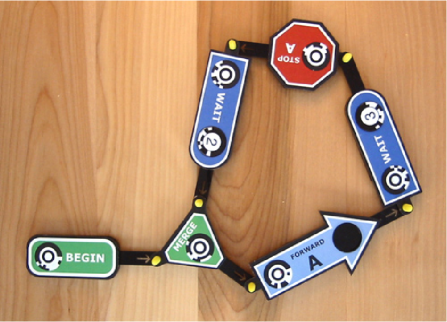
\includegraphics[width=0.6\textwidth]{img/relworks/tern.png}
  \caption{Example Tern statement~\cite{HornRobert:2007}}
  \label{fig:tern}
\end{figure}

Another study~\cite{HornRobert:2007} developed and analyzed a visual
language called \tern. This language is based on the text\hyp{}based
programming language described in the book ``Karel the Robot: A Gentle
Introduction to the Art of Programming''~\cite{Pattis:1994}. In \tern,
students connect wooden blocks shaped like jigsaw puzzle pieces, shown
by~\fig{fig:tern}, form flow\hyp{}of\hyp{}control chains for
elementary virtual robots in a grid world displayed on a computer
screen. Students cooperatively design and create programs on their
desks or on the floor by connecting pieces among each other. These
pieces were scanned by a portable station and a reliable computer
vision software in order to compile the abstracted code. This visual
tool is of special help to incite students towards collaboration. They
program multiple robots that can interact in the same world. Several
teams of students work together to solve the proposed challenges that
include collecting objects and navigating through a maze.

\begin{figure}[h!]
  \centering
  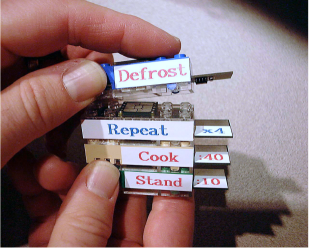
\includegraphics[width=0.6\textwidth]{img/relworks/bricks.png}
  \caption{Tangible programming bricks~\cite{McNerney:2000}}
  \label{fig:bricks}
\end{figure}

Similar to the later, tangible programming bricks~\cite{McNerney:2000}
are physical building blocks for constructing simple programs. These
bricks, which can be observed in~\fig{fig:bricks}, prove to be useful
for controlling diverse objects such as toy cars or kitchen
appliances. This interface brings down the wall that divide
programmers from non\hyp{}programmers by allowing children and novices
to create their own controlling software. The users are encouraged to
adopt it because the bricks are easier to use than text editors, help
to explain to others their programs and to remember better their
programs in comparison to traditional programs.

\begin{figure}
  \centering
  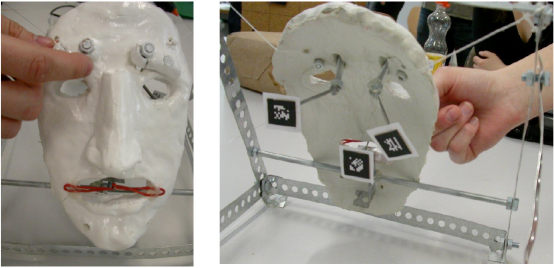
\includegraphics[width=0.8\textwidth]{img/relworks/ar_proto.png}
  \caption{Augmented Reality prototype~\cite{HorneckerPsik:2005}}
  \label{fig:arproto}
\end{figure}

Finally, \emph{augmented reality} (AR) plays an important role in
didactic interfaces. A substantial work has been developed by a group
of teachers and students who created a technique for quick prototyping
of tangible interfaces based on AR~\cite{HorneckerPsik:2005}. The
students creatively adapted optical \artoolkit markers for a class on
experimental prototyping of tangible appliances. The markers are used
to visually track the position of objects, with the advantage of a
wide variety of interactions as the one shown in~\fig{fig:arproto}.
Another work~\cite{Billinghurst:2002} combines the idea of a virtual
guitar assistant with AR. The remarkable part of the system is the
visual warnings displayed when invalid notes are played.

\constructd is a ``three dimensional geometric construction tool
specifically designed for mathematics and geometry
education''~\cite{KaufmannSchmalstieg:2002}. The main contributions of
this research lies in the collaborative environment created around the
interaction of the augmented reality appliances and the concrete
implementation of a virtual 3D scenario for 3D objects. Initial
evaluations show that students work in a constructive manner within
only a short delay. Even though the system has not been deployed in a
production environment, these preliminary results encourage researches
towards the development of augmented reality interfaces with educative
purposes.

%%-*-latex-*-

\section{Methodology}

\noindent\textbf{System overview.} The application challenges the
student to solve a problem by interacting with stacks of blocks placed
on a table. A complete session is best understood as a series of
scenes, that is, snapshots of the board, which abstracts the execution
trace of an \erlang function on a given input, i.e., the initial
setting of the board. Markers are signs that are captured and
recognized by the system from the physical scene. They are
specifically designed to be easily understood by the \artoolkit (which
is a back\hyp{}end for \osgart) and are stuck on each block. They come
in three kinds: \textsl{Item}, \textsl{Stack} and \textsl{Switch}
(whose occultation by the hand triggers a snapshot). For each
recognized marker, a number, a variable, a picture may be superimposed
to the video feed and sent to a monitor. This 3D\hyp{}capable AR
feature is supported by another back\hyp{}end of \osgart called \osg.

\medskip

\noindent\textbf{Interactions.} The stack data structure can be
modified only by two simple operations: pop and push. These are the
minimum set of operations required to allow us to change the data in
any way we wish. However, in our system it is necessary to recognize
the block source and destination, that is, a stack, the table (it then
represents a value which is not a stack) or outside/inside the scene,
so the resulting set of operations is the following:
\begin{itemize}

  \item \textsl{Pop:} moving the top block from a stack onto the
    table;

  \item \textsl{Push}: moving a block from the table onto the top of a
    stack (dual of \textsl{Pop});

  \item \textsl{Pop-Push:} moving a top block from a stack on top of
    another stack (logical composition of \textsl{Pop} and
    \textsl{Push});

  \item \textsl{Discard:} moving a block or stack out of the scene,
    regardless of where it is located;

  \item \textsl{Create:} moving a block or a stack from outside the
    scene onto the table or the top of a stack (dual of
    \textsl{Discard}).
    
\end{itemize}
Changing a scene by any other means or by combining at once two or
more of these operations is considered invalid. These situations are
detected by the application which then stops the session with an error
message explaining what happened and prompts the student to restart
from scratch by placing the blocks back into a valid initial scene.

The system offers two execution modes: one called \emph{free},
allowing the student to freely, but validly, move blocks and another
one called \emph{supervised} in which each operation is checked to
conform to a possible solution, otherwise it is rejected and signalled
by a visual cue.

Adding new problems requires validating initial and final scenes and
dynamically creating \emph{positive scenarios}, that is, admissible
execution traces for different possible \erlang functions
corresponding to the problem. There are currently five problems
defined: stack reversal, joining two stacks, removing all the
occurrences of a given block in a stack, removing all consecutively
repeated blocks and sorting by insertion. The last two exercises are
more than structurally recursive because their assume some property on
the denotations of the blocks, equality and a total order,
respectively.

\bigskip

\noindent\textbf{A session.} Through the interface, blocks augmented
in yellow denote the base of stacks and light blue blocks represent
items belonging to a stack. The block with a camera icon projected
upon stands for the switch that, when hidden, triggers a scene
snapshot. A session ends with the system superimposing a
congratulation message if the student provides a correct and validly
obtained answer. In the case of an invalid action, the system displays
a message indicating the cause of the mistake, the blocks involved in
the invalid move will be augmented with red and the student will have
to restart the session from the beginning.

To illustrate how the interface works, we are going to step through a
sample session of the exercise consisting in joining two stacks, that
is, forming a new stack by moving all the items of one stack onto the
top of another, while retaining their original order. Textually, in
\erlang, this means that, given the stacks \texttt{P} and \texttt{Q},
with \texttt{P} denoting \texttt{[1,2]} (the top is \texttt{1} and the
bottom \texttt{2}) and \texttt{Q} denoting \texttt{[3,4]}, the joining
of \texttt{P} and \texttt{Q} is \texttt{[1,2,3,4]}. The user starts
the session by setting two stacks on the table, representing the input
arguments \texttt{P} (on the left) and \texttt{Q} (on the right) in
\erlang, i.e., \texttt{join(P,Q)} is the function call to
compute. Some random integers are superimposed on the blocks (they are
not random in the coming snapshots, so it is easier to follow the
transformations). This scene can be seen in
Figure~\ref{fig:head1}. 
\begin{figure}[!h]
\centering
\subfloat[\texttt{join([1,2],[3,4])}\label{fig:head1}]{
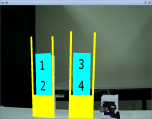
\includegraphics[scale=1.0]{img/step0.png}
}
\quad
\subfloat[\texttt{join([],[1,2],[3,4])}\label{fig:body1}]{
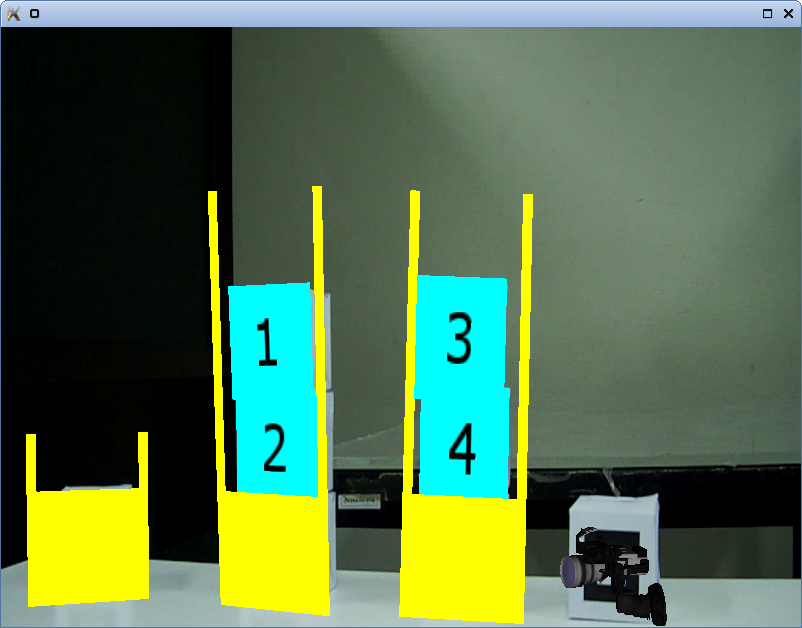
\includegraphics[scale=1.0]{img/step1.png}
}
\caption{\texttt{\small join(P,Q) -> join([],P,Q)}
\label{fig:clause1}}
\end{figure}
The change of scene is denoted in \erlang by an arrow \texttt{->} at
the left of which is a pattern for the current scene and at the right
is the next scene in terms of the previous one. The final result
\texttt{[1,2,3,4]} is shown on the display and the user is prompted to
introduce from outside the scene an empty stack at the leftmost side
of the scene, which will be used as a temporary accumulator (operation
\textsl{Create}). This new scene is in Figure~\ref{fig:body1} and the
\erlang piece of code whose instanciation applies here is {\small
\begin{verbatim}
join(P,Q) -> join([],P,Q).
\end{verbatim}
}
\noindent 
where \texttt{[]} represents the empty stack. The user is now expected
to move top blocks from the middle stack (\texttt{P}) to the left
stack (operation \textsl{Pop\hyp{}Push}), as shown in
Figure~\ref{fig:clause2}.
\begin{figure}[!h]
\centering
\subfloat[\texttt{join([],[1,2],[3,4])}]{
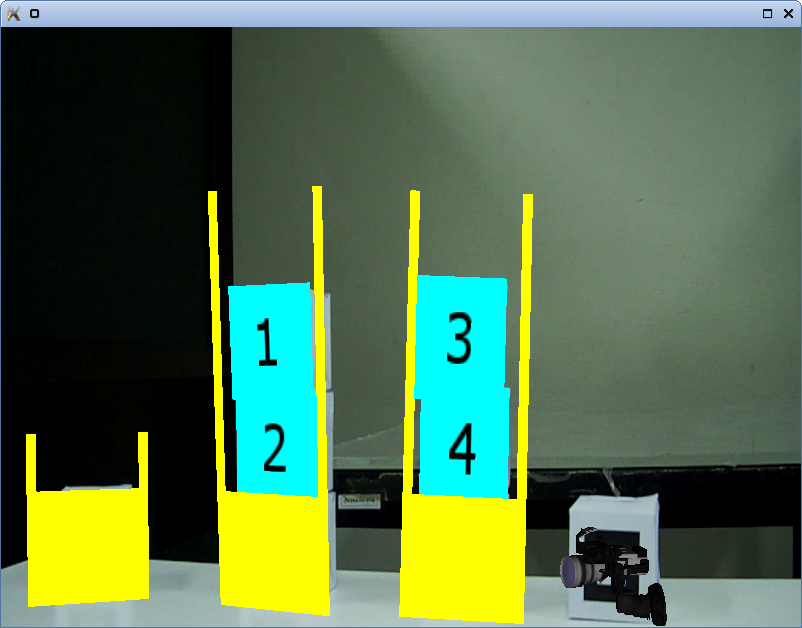
\includegraphics[scale=1.0]{img/step1.png}
}
\quad
\subfloat[\texttt{join([1],[2],[3,4])}]{
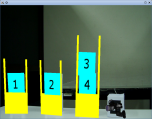
\includegraphics[scale=1.0]{img/step2.png}
}
\caption{\texttt{\small join(A,[I|P],Q) -> join([I|A],P,Q)}
\label{fig:clause2}}
\end{figure}
This transformation is captured by the \erlang clause
{\small
\begin{verbatim}
join(A,[I|P],Q) -> join([I|A],P,Q);
\end{verbatim}
}
\noindent In \erlang, \texttt{[I|P]} is a pattern which matches any
non\hyp{}empty stack whose top block is named \texttt{I} and the
remaining stack \texttt{P}. After repeating this operation one more
time on our example, the scene is as shown in Figure~\ref{fig:head3}.
\begin{figure}[!h]
\centering
\subfloat[\texttt{join([2,1],[],[3,4])}\label{fig:head3}]{
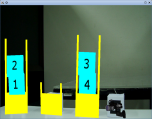
\includegraphics[scale=1.0]{img/step3.png}
}
\quad
\subfloat[\texttt{join([1],[],[2,3,4])}\label{fig:body3}]{
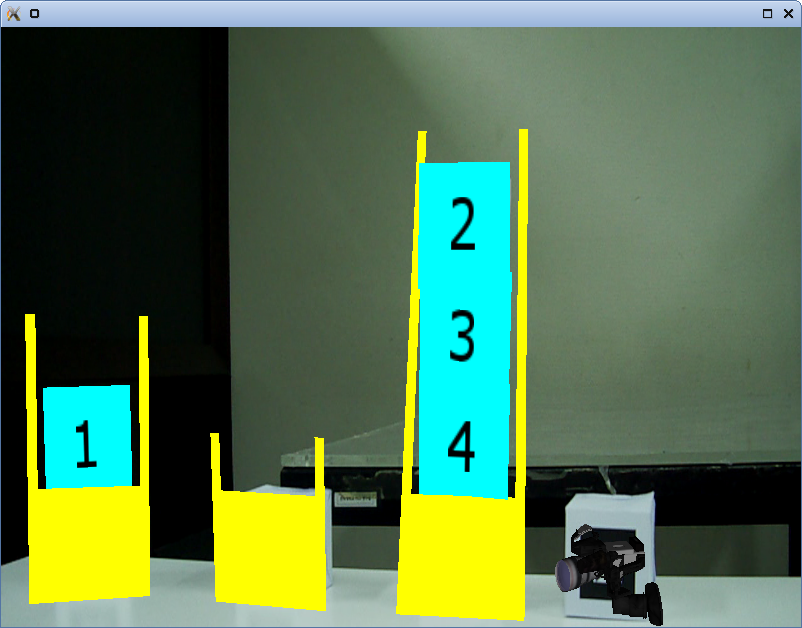
\includegraphics[scale=1.0]{img/step4.png}
}
\caption{\texttt{\small join([I|A],[],Q) -> join(A,[],[I|Q])}
\label{fig:clause3}}
\end{figure}
It is matched by the pattern \texttt{join([I|A],[],Q)}, meaning ``left
stack with top block \texttt{I} and sub\hyp{}stack \texttt{A}, middle
stack empty and right stack \texttt{Q} unchanged.'' The next phase
consists in moving the blocks from the leftmost stack to the rightmost
(operation \textsl{Pop\hyp{}Push}). This is shown in
Figure~\ref{fig:clause3}, which corresponds to an instance of the
piece of source code 
{\small
\begin{verbatim}
join([I|A],[],Q) -> join(A,[],[I|Q]);
\end{verbatim}
}
\noindent After repeating this operation once more on our example, the
left stack becomes empty and the corresponding scene is seen in
Figure~\ref{fig:head4}. 
\begin{figure}[!h]
\centering
\subfloat[\texttt{join([],[],[1,2,3,4])}\label{fig:head4}]{
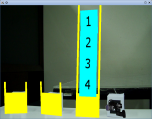
\includegraphics[scale=1.0]{img/step5.png}
}
\quad
\subfloat[\texttt{[2,3,4]}\label{fig:body4}]{
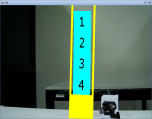
\includegraphics[scale=1.0]{img/step6.png}
}
\caption{\texttt{\small join([],[],Q) -> Q}}
\label{fig:clause4}
\end{figure}
The \erlang pattern for it is \texttt{join([],[],Q)}. The result is
finally reached by keeping only the non\hyp{}empty stack on the scene
(operation \textsl{Discard} twice), as shown in
Figure~\ref{fig:clause4}. This is expressed by the clause
{\small
\begin{verbatim}
join([],[],Q) -> Q.
\end{verbatim}
} 
The student is not presented the \erlang at this stage, we wanted to
show the analogy between the AR scene and the textual program, which
the student in a later session will be asked to write directly. Here,
the complete \erlang program of this session was as follows (module
declarations omitted):
{\small
\begin{verbatim}
join(          P,Q) -> join(   [], P,    Q).
join(    A,[I|P],Q) -> join([I|A], P,    Q);
join([I|A],   [],Q) -> join(    A,[],[I|Q]);
join(   [],   [],Q) -> Q.
\end{verbatim}
}

\medskip

\noindent\textbf{Scope and limitations.} From the standpoint of
programming expressivity, the system is limited to functions based on
structural recursion on stacks and constant values. This is a
consequence of using a TUI, so adding new interactions would require
technologies that are not widely spread, for example gesture
recognition, motion tracking, voice recognition, etc. On the other
hand, with the current system, it just as easy to use rectangular
pieces of paper on a table instead of blocks, making it as portable as
the laptop with a webcam running it. The set of definable function is
also restricted to tail\hyp{}recursivity because representing the
control stack would require a special stack growing top\hyp{}down, so
the order of the instances of the control contexts is preserved. Since
the system is intended to be used by novices as a temporary tool to
understand simple cases of recursion, instead of as a general
programming environment, this is not an impediment.

\medskip

\noindent\textbf{Future experiments.} The first phase is made up of
three stages, which are repeated. In a first stage, the students will
be asked to build some stacks and randomly chosen integers will be
displayed on the blocks, one per block. The expected result will in
turn be shown on the screen. The student may select either the free or
supervised execution mode and try to reach the goal. After, two more
random examples for the same problem will be proposed. This stage
relies only on \emph{concrete examples}, as the one illustrated above
with \texttt{join}. It presents some similarities with the framework
of \emph{programming by example}, except that the goal is not to teach
the computer how to program but the other way round.

In the second stage, another random example for the same problem is
displayed but only the top of the stacks will be visible. This is
meant to induce in the learner the understanding that the exercise can
be solved without relying on global knowledge and that
\emph{information hiding} actually helps to focus the attention on the
smallest part of the data which is needed to make one more little step
towards the result. Each time a \textsl{Push\hyp{}Pop} operation is
performed, for instance, only the topmost blocks are consistently
shown.

After three runs like this, three other examples of the same problem
are offered, but instead of integers superimposed on the block
markers, \emph{variables} are. This last stage aims at giving rise to
\emph{abstraction} and prepares the transfer to textual programming.

When the last stage is over, another problem is submitted to the
student etc. until the interface hopefully becomes useless and the
direct programming of the \erlang functions corresponding to the
previous exercises is attempted. In the second phase, the professor
shows the analogy between, on the one hand, the stacks of blocks and
the valid operations learnt by means of the interface and, on the
other hand, the \erlang syntax for lists and the \erlang semantics. We
expect to measure a statistically significant transfer of training for
students who used the system in comparison with students who did not.


%%-*-latex-*-

%*******************************************************************************
\section{Test Cases}\label{sec:testcases}
%*******************************************************************************

In order to validate these points five problems have been implemented:
\emph{Reverse}, \emph{Join}, \emph{Remove all}, \emph{Compress} and
\emph{Insertion sort}. \emph{Reverse} consists in rearrange the items
of an input list in the opposite order. The student is expected to
create an empty temporary list and proceed to pop the elements from
the original input list and push them into the temporary list. The
effect of popping and pushing items among lists will cause the
resulting elements to be in reverse order as it is required. The next
exercise consists in \emph{joining} two stacks, that is, forming a new
stack by moving all the items of one stack onto the top of another,
while retaining their original order. Another is \emph{Remove all},
which objective is to purge the items from a list that are equal to
a given value, the list must preserve its initial order. Similar to
the latter is \emph{Compress}, where consecutive repeated elements of
an input list are to be removed. Finally, the most interesting
problem, \emph{Insertion sort}, where an input list must be
reorganized in ascending numerical order. The problems where choose
because each one provide different levels of difficult, being Join the
easiest and Insertion sort the hardest. Hence, the student can adapt
to the system in a progressive way.

\newcommand\stepfig[5]{
  \subfigure[{\scriptsize\texttt{#1}} {\scriptsize(#2)}]
            {\includegraphics[width=0.45\textwidth]{img/#4/#3/#3#5.png}\label{fig:#3:#4:#5}}
}

%*******************************************************************************
\subsection{Reverse}
%*******************************************************************************

\renewcommand*\FancyVerbStartString{BEGIN-REV}
\renewcommand*\FancyVerbStopString{END-REV}
\begin{figure}[h!]
  \fvset{frame=leftline,numbers=left,firstnumber=1,xleftmargin=3ex}
  \VerbatimInput{testcases.erl}
  \caption{Reverse source code}
  \label{fig:code:rev}
\end{figure}

This is the most simple problem. The student will start the
interaction by placing one list with at least two elements on the
table. The second step consists in creating a temporary list \emph{T}
and afterward moving the items one by one from the input list into
\emph{T}. The last step is to remove the initial list once it is
empty. The \erlang code representation of this problem can be seen
in~\fig{fig:code:rev}.

\begin{figure}[h!]
  \centering
  \stepfig{reverse(L)}{1}{rev}{p1}{1}
  \stepfig{reverse(L,[])}{1}{rev}{p1}{2}
  \stepfig{reverse(L,[I\textbar T])}{2}{rev}{p1}{3}
  \stepfig{reverse([I\textbar L],T)}{2}{rev}{p1}{4}
  \stepfig{reverse([],T)}{3}{rev}{p1}{5}
  \stepfig{T}{3}{rev}{p1}{6}
  \caption{Reverse in the first didactic phase}
\end{figure}

\FloatBarrier

\Fig{fig:rev:p1:1} shows a concrete step by step interaction when
\emph{L} denotes \texttt{[1, 2, 3]} where \texttt{1} is the head and
\texttt{[2, 3]} is the tail. Its counterparts of the second and third
phases are shown in~\fig{fig:rev:p2:1} and in~\fig{fig:rev:p3:1}
respectively.

\begin{figure}[h!]
  \centering
  \stepfig{reverse(L)}{1}{rev}{p2}{1}
  \stepfig{reverse(L,[])}{1}{rev}{p2}{2}
  \stepfig{reverse(L,[I\textbar T])}{2}{rev}{p2}{3}
  \stepfig{reverse([I\textbar L],T)}{2}{rev}{p2}{4}
  \stepfig{reverse([],T)}{3}{rev}{p2}{5}
  \stepfig{T}{3}{rev}{p2}{6}
  \caption{Reverse in the second didactic phase}
\end{figure}

\FloatBarrier

\begin{figure}[h!]
  \centering
  \stepfig{reverse(L)}{1}{rev}{p3}{1}
  \stepfig{reverse(L,[])}{1}{rev}{p3}{2}
  \stepfig{reverse(L,[I\textbar T])}{2}{rev}{p3}{3}
  \stepfig{reverse([I\textbar L],T)}{2}{rev}{p3}{4}
  \stepfig{reverse([],T)}{3}{rev}{p3}{5}
  \stepfig{T}{3}{rev}{p3}{6}
  \caption{Reverse in the third didactic phase}
\end{figure}

In the first step, a temporary list \emph{T} is created as shown by
the movement from~\figs{fig:rev:p1:1}{fig:rev:p1:2} and also in
the~\figs{fig:rev:p2:1}{fig:rev:p2:2}
and~\figs{fig:rev:p3:1}{fig:rev:p3:2}. Steps two, three and four
consists of moving the items into the new list, these are equivalent
to the line 2 of the \erlang statement of~\fig{fig:code:rev} and also
to~\figs{fig:rev:p1:3}{fig:rev:p1:5}. Here, the contents of \emph{T}
change from an empty list to \texttt{[3]}, then, in the third step to
\texttt{[3, 2]} and \texttt{[3, 2, 1]} in the fourth step.

Finally, \fig{fig:rev:p1:6} illustrates the discard of the \emph{L}
list. At this point, the temporary lists contains the answer to the
problem.

\FloatBarrier
%*******************************************************************************
\subsection{Join}
%*******************************************************************************

\renewcommand*\FancyVerbStartString{BEGIN-JOIN}
\renewcommand*\FancyVerbStopString{END-JOIN}
\begin{figure}[h!]
  \fvset{frame=leftline,numbers=left,firstnumber=1,xleftmargin=3ex}
  \VerbatimInput{testcases.erl}
  \caption{Join source code}
  \label{fig:code:join}
\end{figure}

Initially, the user will set two lists, \emph{L} and \emph{M}, on the
table, each with two or more items as seen in~\fig{fig:join:p3:1}.
The followed actions consist in doing \poppush of the elements of
\emph{M} into a temporary list leading to a list with reverse order,
this step can be seen in~\figs{fig:join:p3:2}{fig:join:p3:4}. Moving
the items of this list on top of \emph{L},
as~\figs{fig:join:p3:5}{fig:join:p3:6} show, will give the expected
result. Thereafter, the final step is to discard both the temporary
list and \emph{M}. This is represented in the code
of~\fig{fig:code:join}.

\begin{figure}[h!]
  \centering
  \stepfig{join(L,M)}{1}{join}{p1}{1}
  \stepfig{join(L,M,[])}{1}{join}{p1}{2}
  \stepfig{join(L,[I\textbar M],T)}{2}{join}{p1}{3}
  \stepfig{join(L,M,[I\textbar T])}{2}{join}{p1}{4}
  \stepfig{join(L,[],[I\textbar T])}{3}{join}{p1}{5}
  \stepfig{join(L,[],[])}{4}{join}{p1}{6}
  \stepfig{L}{4}{join}{p1}{7}
  \caption{Join in the first didactic phase}
\end{figure}

\begin{figure}[h!]
  \centering
  \stepfig{join(L,M)}{1}{join}{p2}{1}
  \stepfig{join(L,M,[])}{1}{join}{p2}{2}
  \stepfig{join(L,[I\textbar M],T)}{2}{join}{p2}{3}
  \stepfig{join(L,M,[I\textbar T])}{2}{join}{p2}{4}
  \stepfig{join(L,[],[I\textbar T])}{3}{join}{p2}{5}
  \stepfig{join(L,[],[])}{4}{join}{p2}{6}
  \stepfig{L}{4}{join}{p2}{7}
  \caption{Join in the second didactic phase}
  \label{fig:join:p2}
\end{figure}

\begin{figure}[h!]
  \centering
  \stepfig{join(L,M)}{1}{join}{p3}{1}
  \stepfig{join(L,M,[])}{1}{join}{p3}{2}
  \stepfig{join(L,[I\textbar M],T)}{2}{join}{p3}{3}
  \stepfig{join(L,M,[I\textbar T])}{2}{join}{p3}{4}
  \stepfig{join(L,[],[I\textbar T])}{3}{join}{p3}{5}
  \stepfig{join(L,[],[])}{4}{join}{p3}{6}
  \stepfig{L}{4}{join}{p3}{7}
  \caption{Join in the third didactic phase}
\end{figure}

In a trivial exercise the student is given two input lists denoting
\texttt{[3, 4]} and \texttt{[1, 2]} as \emph{L} and \emph{M}
respectively. \Figs{fig:join:p1:1}{fig:join:p1:2} show the creation of the
temporary list \emph{T} and~\figs{fig:join:p1:3}{fig:join:p1:4} show how the
items of \emph{M} must be dumped into \emph{T}, which, because of the
movements, is now composed of \texttt{[2, 1]}.

When \emph{T} is emptied out on top of \emph{L}, as seen
in the~\figs{fig:join:p1:5}{fig:join:p1:6} or line 3 of the code
of~\fig{fig:code:join}, \emph{T} and \emph{M} will then have no
contents and on the other side \emph{L} will contain
\texttt{[1, 2, 3, 4]}. For this reason, the final step
of~\fig{fig:join:p1:7} consists in discarding these empty lists,
highlighting \emph{L} as the solution.

The two final steps are represented in \erlang code in the lines 3
and 4 of~\fig{fig:code:join} and also in the second didactic phase in
the~\fig{fig:join:p2}.

\FloatBarrier
%*******************************************************************************
\subsection{Remove All} \label{sec:removeall}
%*******************************************************************************

\renewcommand*\FancyVerbStartString{BEGIN-REMALL}
\renewcommand*\FancyVerbStopString{END-REMALL}
\begin{figure}[h!]
  \fvset{frame=leftline,numbers=left,firstnumber=1,xleftmargin=3ex}
  \VerbatimInput{testcases.erl}
  \caption{Remove All source code}
  \label{fig:code:remall}
\end{figure}

\begin{figure}[h!]
  \centering
  \stepfig{remall(L,E)}{1}{remall}{p1}{1}
  \stepfig{remall([I\textbar L],E,T,P)}{5}{remall}{p1}{2}
  \stepfig{remall(L,E,[I\textbar T],P)}{5}{remall}{p1}{3}
  \stepfig{remall([E\textbar L],E,T,P)}{4}{remall}{p1}{4}
  \stepfig{remall(L,E,T,P)}{4}{remall}{p1}{5}
  \stepfig{remall([],E,[I\textbar T],P)}{3}{remall}{p1}{6}
  \stepfig{remall([],\_,[],P)}{2}{remall}{p1}{7}
  \stepfig{P}{2}{remall}{p1}{8}
  \caption{Remove All in the first didactic phase}
\end{figure}

In \emph{Remove all} the elements of an input stack \emph{L} are
eliminated when they are equal to a base value \emph{E}. In order to
solve this, the student will create two temporary lists \emph{T} and
\emph{P} respectively. The next step is conditional, \emph{L}'s top
element must be discarded when it is equals to \emph{E}, otherwise
it must be moved on top of the \emph{T} stack. Once \emph{L} contains
no items, \emph{T} elements have to be dump into \emph{P}. \emph{P}
will be the solution at the end of this process, thus, \emph{E},
\emph{L} and \emph{T} must be discarded. The \erlang code
representation of this problem is shown in~\fig{fig:code:remall}.

\begin{figure}[h!]
  \centering
  \stepfig{remall(L,E)}{1}{remall}{p2}{1}
  \stepfig{remall([I\textbar L],E,T,P)}{5}{remall}{p2}{2}
  \stepfig{remall(L,E,[I\textbar T],P)}{5}{remall}{p2}{3}
  \stepfig{remall([E\textbar L],E,T,P)}{4}{remall}{p2}{4}
  \stepfig{remall(L,E,T,P)}{4}{remall}{p2}{5}
  \stepfig{remall([],E,[I\textbar T],P)}{3}{remall}{p2}{6}
  \stepfig{remall([],\_,[],P)}{2}{remall}{p2}{7}
  \stepfig{P}{2}{remall}{p2}{8}
  \caption{Remove All in the second didactic phase}
  \label{fig:remall:p2}
\end{figure}

To exemplify this problem, the data \texttt{[1, 2, 3]} and the base
value \texttt{3} represent the input parameters \emph{L} and
\emph{E} respectively.

This exercise requires two intermediary lists
which are created between the~\figs{fig:remall:p1:1}{fig:remall:p1:2}. After
this, a conditional statement takes place, this is, \emph{L} items
equals to \texttt{3} must be discarded, the rest of the items must be
pushed into \emph{T}. \Figs{fig:remall:p1:4}{fig:remall:p1:5} show how the
item \texttt{3} is discarded and~\fig{fig:remall:p1:4} shows how the
items \texttt{1} and \texttt{2} are pushed into \emph{T}. The first
condition is corresponded in \erlang code in the line 4
of~\fig{fig:code:remall} and the second in the line 5.

\begin{figure}[h!]
  \centering
  \stepfig{remall(L,E)}{1}{remall}{p3}{1}
  \stepfig{remall([I\textbar L],E,T,P)}{5}{remall}{p3}{2}
  \stepfig{remall(L,E,[I\textbar T],P)}{5}{remall}{p3}{3}
  \stepfig{remall([E\textbar L],E,T,P)}{4}{remall}{p3}{4}
  \stepfig{remall(L,E,T,P)}{4}{remall}{p3}{5}
  \stepfig{remall([],E,[I\textbar T],P)}{3}{remall}{p3}{6}
  \stepfig{remall([],\_,[],P)}{2}{remall}{p3}{7}
  \stepfig{P}{2}{remall}{p3}{8}
  \caption{Remove All in the third didactic phase}
  \label{fig:remall:p3}
\end{figure}

When \emph{L} is empty \emph{T} items, \texttt{[2, 1]} are dumped into
\emph{P} as seen in~\figs{fig:remall:p1:5}{fig:remall:p1:7} and line 3
of~\fig{fig:code:remall}. Subsequently, is necessary to discard the
left over elements: \emph{E}, \emph{L} and \emph{T}. The final result
is then \texttt{[1, 2]} contained in \emph{P}, this step is shown
in~\fig{fig:remall:p1:8}. This full example can be seen
in~\fig{fig:remall:p2} and~\fig{fig:remall:p3} as it is represented in
the second and third phase respectively.

\FloatBarrier
%*******************************************************************************
\subsection{Compress}
%*******************************************************************************

\renewcommand*\FancyVerbStartString{BEGIN-COMPRESS}
\renewcommand*\FancyVerbStopString{END-COMPRESS}
\begin{figure}[h!]
  \fvset{frame=leftline,numbers=left,firstnumber=1,xleftmargin=3ex}
  \VerbatimInput{testcases.erl}
  \caption{Compress source code}
  \label{fig:code:compress}
\end{figure}

\emph{Compress} consists in eliminating the consecutively repeated
elements from a stack \emph{L}. This exercise is logically similar
to \vref{sec:removeall} because items \emph{flow} with the same
pattern. The main differences lies in the condition of the second step
as here the items are compared with each other instead of to a base
value.

First two temporary stacks \emph{T} and \emph{P} must be
created as seen in~\fig{fig:compress:p3:1}. Second, the user must
proceed to move \emph{L}'s items into \emph{T}, except when the
element is equal to \emph{T}'s top element as in
the~\figs{fig:compress:p3:2}{fig:compress:p3:5}. The third step, as
shown by~\figs{fig:compress:p3:5}{fig:compress:p3:7}, is to dump
\emph{T} into \emph{P} and as a final step \emph{L} and \emph{T}
must be discarded. The non\hyp{}optimized \erlang code representation
of this problem is shown by~\fig{fig:code:compress}

\begin{figure}[h!]
  \centering
  \stepfig{compress(L)}{1}{compress}{p1}{1}
  \stepfig{compress(L,[],[])}{1}{compress}{p1}{2}
  \stepfig{compress([I\textbar L],T,P)}{5}{compress}{p1}{3}
  \stepfig{compress([I\textbar L],[I\textbar T],P)}{4}{compress}{p1}{4}
  \stepfig{compress(L,[I\textbar T],P)}{4}{compress}{p1}{5}
  \stepfig{compress([],T,[I\textbar P])}{3}{compress}{p1}{6}
  \stepfig{compress([],[],P)}{2}{compress}{p1}{7}
  \stepfig{P}{2}{compress}{p1}{8}
  \caption{Compress in the first didactic phase}
\end{figure}

\begin{figure}[h!]
  \centering
  \stepfig{compress(L)}{1}{compress}{p2}{1}
  \stepfig{compress(L,[],[])}{1}{compress}{p2}{2}
  \stepfig{compress([I\textbar L],T,P)}{5}{compress}{p2}{3}
  \stepfig{compress([I\textbar L],[I\textbar T],P)}{4}{compress}{p2}{4}
  \stepfig{compress(L,[I\textbar T],P)}{4}{compress}{p2}{5}
  \stepfig{compress([],T,[I\textbar P])}{3}{compress}{p2}{6}
  \stepfig{compress([],[],P)}{2}{compress}{p2}{7}
  \stepfig{P}{2}{compress}{p2}{8}
  \caption{Compress in the second didactic phase}
\end{figure}

\begin{figure}[h!]
  \centering
  \stepfig{compress(L)}{1}{compress}{p3}{1}
  \stepfig{compress(L,[],[])}{1}{compress}{p3}{2}
  \stepfig{compress([I\textbar L],T,P)}{5}{compress}{p3}{3}
  \stepfig{compress([I\textbar L],[I\textbar T],P)}{4}{compress}{p3}{4}
  \stepfig{compress(L,[I\textbar T],P)}{4}{compress}{p3}{5}
  \stepfig{compress([],T,[I\textbar P])}{3}{compress}{p3}{6}
  \stepfig{compress([],[],P)}{2}{compress}{p3}{7}
  \stepfig{P}{2}{compress}{p3}{8}
  \caption{Compress in the third didactic phase}
\end{figure}

The input list \texttt{[1, 3, 3]} is probably the easiest version of
this exercise. Using this input, the first step, as seen
in~\figs{fig:compress:p1:1}{fig:compress:p1:2} is to create two lists
\emph{T} and \emph{P}.

\Figs{fig:compress:p1:4}{fig:compress:p1:5} exemplifies the condition of
line 4 of the \erlang code in~\fig{fig:code:compress} where the top
item of the input list is removed for being equal to the top of
\emph{T}. On the other hand, \figs{fig:compress:p1:3}{fig:compress:p1:4}
correspond to the line 5 of the same code which consists in moving
the elements that does not match the condition of the previous step.
Once the input list is empty the content of \emph{T} is:
\texttt{[3, 1]}, this is, a reverse view of the initial elements minus
the ones consecutively repeated.

Finally, dumping \emph{T} on top of \emph{P}, as seen
in~\figs{fig:compress:p1:5}{fig:compress:p1:7} and which logic process
can be seen in line 3 of~\fignov{fig:code:compress}, will lead to the final
answer shown in~\fignov{fig:compress:p1:8}: \texttt{[1, 3]}.

\FloatBarrier
%*******************************************************************************
\subsection{Insertion Sort}
%*******************************************************************************

\emph{Sorting} consists in arranging the items of a list in a given
order. Sorting algorithms are always present in introductory
programming classes where the wide variety of solutions to the problem
is a good base to present common concepts like
\emph{divide\hyp{}and\hyp{}conquer strategy}, computational
delay analysis, asymptotics, etc. Its pervasiveness in
real\hyp{}life situations makes it a highly studied problem.

\renewcommand*\FancyVerbStartString{BEGIN-ISORT}
\renewcommand*\FancyVerbStopString{END-ISORT}
\begin{figure}
  \fvset{frame=leftline,numbers=left,firstnumber=1,xleftmargin=3ex}
  {\footnotesize \VerbatimInput{testcases.erl}}
  \caption{Insertion Sort source code}
  \label{fig:code:isort}
\end{figure}

For the sake of simplicity, the experiment focuses on ascending
numerical order with \emph{insertion sort}. Regarding of computational
delay and memory usage, insertion sort is not the most optimum.
However, it is simple and plain, thus, perfectly suitable for
novices in recursion.

\begin{figure}[h!]
  \centering
  \stepfig{isort(L)}{1}{isort}{p1}{1}
  \stepfig{isort(L,[],[])}{1}{isort}{p1}{2}
  \stepfig{isort([I\textbar L],P,[K\textbar Q]) when K>I}{4}{isort}{p1}{3}
  \stepfig{isort([I\textbar L],[K\textbar P],Q)}{4}{isort}{p1}{4}
  \stepfig{isort([I\textbar L],[J\textbar P],Q) when I>J}{5}{isort}{p1}{5}
  \stepfig{isort([I\textbar L],P,[J\textbar Q])}{5}{isort}{p1}{6}
  \stepfig{isort([I\textbar L],P,[K\textbar Q]) when K>I}{4}{isort}{p1}{7}
  \stepfig{isort([I\textbar L],[K\textbar P],Q)}{4}{isort}{p1}{8}
  \caption{Insertion Sort in the first didactic phase (Part 1/2)}
\end{figure}

\begin{figure}[h!]
  \centering
  \stepfig{isort([I\textbar L],[K\textbar P],Q)}{4}{isort}{p1}{9}
  \stepfig{isort([I\textbar L],P,Q)}{6}{isort}{p1}{10}
  \stepfig{isort(L,P,[I\textbar Q])}{6}{isort}{p1}{11}
  \stepfig{isort([],[J\textbar P],Q)}{3}{isort}{p1}{12}
  \stepfig{isort([],P,[J\textbar Q])}{3}{isort}{p1}{13}
  \stepfig{isort([],[],Q)}{2}{isort}{p1}{14}
  \stepfig{Q}{2}{isort}{p1}{15}
  \caption{Insertion Sort in the first didactic phase (Part 2/2)}
\end{figure}

\begin{figure}[h!]
  \centering
  \stepfig{isort(L)}{1}{isort}{p2}{1}
  \stepfig{isort(L,[],[])}{1}{isort}{p2}{2}
  \stepfig{isort([I\textbar L],P,[K\textbar Q]) when K>I}{4}{isort}{p2}{3}
  \stepfig{isort([I\textbar L],[K\textbar P],Q)}{4}{isort}{p2}{4}
  \stepfig{isort([I\textbar L],[J\textbar P],Q) when I>J}{5}{isort}{p2}{5}
  \stepfig{isort([I\textbar L],P,[J\textbar Q])}{5}{isort}{p2}{6}
  \stepfig{isort([I\textbar L],P,[K\textbar Q]) when K>I}{4}{isort}{p2}{7}
  \stepfig{isort([I\textbar L],[K\textbar P],Q)}{4}{isort}{p2}{8}
  \caption{Insertion Sort in the second didactic phase (Part 1/2)}
\end{figure}

\begin{figure}[h!]
  \centering
  \stepfig{isort([I\textbar L],[K\textbar P],Q)}{4}{isort}{p2}{9}
  \stepfig{isort([I\textbar L],P,Q)}{6}{isort}{p2}{10}
  \stepfig{isort(L,P,[I\textbar Q])}{6}{isort}{p2}{11}
  \stepfig{isort([],[J\textbar P],Q)}{3}{isort}{p2}{12}
  \stepfig{isort([],P,[J\textbar Q])}{3}{isort}{p2}{13}
  \stepfig{isort([],[],Q)}{2}{isort}{p2}{14}
  \stepfig{Q}{2}{isort}{p2}{15}
  \caption{Insertion Sort in the second didactic phase (Part 2/2)}
  \label{fig:isort:p2}
\end{figure}

\begin{figure}[h!]
  \centering
  \stepfig{isort(L)}{1}{isort}{p3}{1}
  \stepfig{isort(L,[],[])}{1}{isort}{p3}{2}
  \stepfig{isort([I\textbar L],P,[K\textbar Q]) when K>I}{4}{isort}{p3}{3}
  \stepfig{isort([I\textbar L],[K\textbar P],Q)}{4}{isort}{p3}{4}
  \stepfig{isort([I\textbar L],[J\textbar P],Q) when I>J}{5}{isort}{p3}{5}
  \stepfig{isort([I\textbar L],P,[J\textbar Q])}{5}{isort}{p3}{6}
  \stepfig{isort([I\textbar L],P,[K\textbar Q]) when K>I}{4}{isort}{p3}{7}
  \stepfig{isort([I\textbar L],[K\textbar P],Q)}{4}{isort}{p3}{8}
  \caption{Insertion Sort in the third didactic phase (Part 1/2)}
\end{figure}

\begin{figure}[h!]
  \centering
  \stepfig{isort([I\textbar L],[K\textbar P],Q)}{4}{isort}{p3}{9}
  \stepfig{isort([I\textbar L],P,Q)}{6}{isort}{p3}{10}
  \stepfig{isort(L,P,[I\textbar Q])}{6}{isort}{p3}{11}
  \stepfig{isort([],[J\textbar P],Q)}{3}{isort}{p3}{12}
  \stepfig{isort([],P,[J\textbar Q])}{3}{isort}{p3}{13}
  \stepfig{isort([],[],Q)}{2}{isort}{p3}{14}
  \stepfig{Q}{2}{isort}{p3}{15}
  \caption{Insertion Sort in the third didactic phase (Part 2/2)}
  \label{fig:isort:p3}
\end{figure}

The student is expected to start by creating two temporary lists
\emph{A} and \emph{D} as seen in~\figs{fig:isort:p1:1}{fig:isort:p1:2}.
For a better understanding, the following logic rules must be
considered: \emph{A} has the special property of always being in
ascending order, as for \emph{D}, its elements will persistently be in
descending order. Therefore, The goal consists in trespassing the
elements from the initial list \emph{L} into \emph{A} by obeying these
rules.

All in all, \emph{D} will be used as an exchange mechanism
to dump \emph{A}'s items when pushing a new item on it would break the
first rule. This process is show by~\fig{fig:isort:p3}.

\emph{L}'s items, must be pushed into \emph{A} only on three cases:
(1) when \emph{A} is an empty list, as
in~\figs{fig:isort:p1:2}{fig:isort:p1:3}; (2) when \emph{D} is an empty list
and the item is greater than \emph{A}'s top, as seen
in~\figs{fig:isort:p1:6}{fig:isort:p1:7}; and (3) when the item is greater
than \emph{A}'s top and lower than \emph{D}'s top, as shown
by~\figs{fig:isort:p1:4}{fig:isort:p1:5}. Respectively, this condition is
stated in~\fig{fig:code:isort} in lines 2, 5 and the clause formed by
lines 6 and 7.

As shown in lines 3 and 4 of the code in~\fig{fig:code:isort}, if the
item is lower than \emph{A}'s top, then \emph{A}'s elements must be
dumped into \emph{D} until one of the firsts conditions is met. In the
given exercise this is seen several times, first
in~\figsnov{fig:isort:p1:3}{fig:isort:p1:4} and then repeatedly
in~\figs{fig:isort:p1:7}{fig:isort:p1:10}.

Line 8 of the code states
that if at any given point the top item of the input list is bigger
than \emph{A}'s top and at the same time bigger than \emph{D}'s top
then \emph{D}'s items must be dumped back into \emph{A} until one
of the three conditions is met. An example of this situation can be
observed in~\figs{fig:isort:p1:5}{fig:isort:p1:6} and later in the steps
of~\figs{fig:isort:p1:11}{fig:isort:p1:14}.

Finally, when the original list is empty all of \emph{D}'s items must
be pushed into \emph{A}, then, the final step is to discard the
initial list and \emph{D}, like shown
in~\figs{fig:isort:p1:14}{fig:isort:p1:15} and coded in the line 9.
The~\fig{fig:code:isort} shows the complete \erlang representation of
the previous process and~\fig{fig:isort:p2} shows the process of the
second didactic phase.

\FloatBarrier

%%-*-latex-*-

%*******************************************************************************
\section{Evaluation}
%*******************************************************************************

One of the key concepts to be evaluated, with a focus on recursion, is
the hypothesis that novices would build abstract models more easily
when they experiment with tangible interfaces due to their didactic
virtues.

On this test, special interests has been putted on how lists work,
and, more specifically, how the their contents change through time
when exposed to recursive processes. The block\hyp{}world analogy is
expected to help understand the concept of list by physically
representing its main operations: \pop and \push and its LIFO (Last
Input First Output) behavior. Lists are then, the main data structure
in which recursion bases are built.

%*******************************************************************************
\subsection{Process}
%*******************************************************************************

The evaluation process is conducted with the help of 11 participants,
students from the faculties of Computer Science and Information
Technologies at Konkuk University. Their experience with functional
programming languages and concepts is very varied. Some of them had
never learn recursion or even wrote code in a functional language,
some others can be considered beginners and a final group are students
of the course of programming languages for postgraduates which is
focused on recursion by using \erlang.

The test consists in two parts. The first phase requires each
participant to solve the five exercises described in the section
\vref{sec:testcases}. The second phase is an exploratory survey that
participants are asked to complete.

The assistants are expected to complete the five exercises after a
brief explanation of how the interaction must be done. For simplicity
purposes the input of the problems does not contains more than 4 items
for each list, this means that they will be easy to solve. Only the
first exercise, \emph{Reverse}, is fully guided by a tutor who
explains the interactive process, provides additional information of
invalid actions and a course to follow. This means that \emph{Join},
\emph{Remove all}, \emph{Compress} and \emph{Insertion sort} are to be
solved entirely by the participant, the tutor is a supervisor during
these.

Finally, the survey is used to gather further information related to
the participant opinion of his experience and of the interface. An
introductory section has questions about previous knowledge of
recursion and functional programming. The main part of the
survey contains questions related to the participant experience with
the interface. Finally, the last part concludes with his personal
opinion of the interface and its benefits.

%*******************************************************************************
\subsection{Results}
%*******************************************************************************

The test is conducted in a total period of two weeks, each
participant's session lasts around 20 to 30 minutes and taking in
average 5 minutes per exercise. However, they do not have any time
constraint. After the experiment, several observations were made.

\begin{figure}
  \centering
  \subfigure{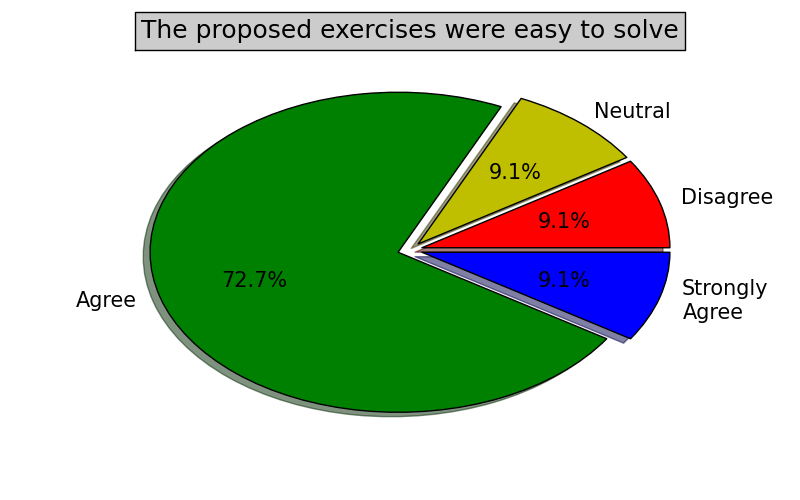
\includegraphics[width=0.47\textwidth]{img/survey/q4.png}\label{fig:survey:q4}}
  \subfigure{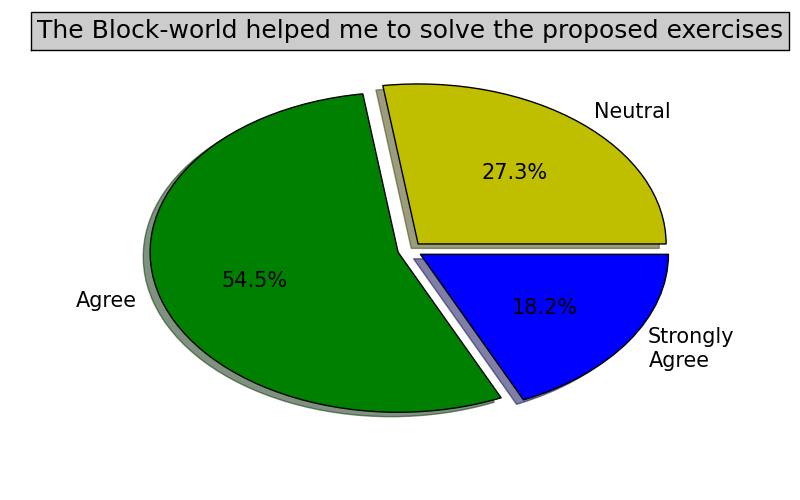
\includegraphics[width=0.47\textwidth]{img/survey/q5.png}\label{fig:survey:q5}}
  \subfigure{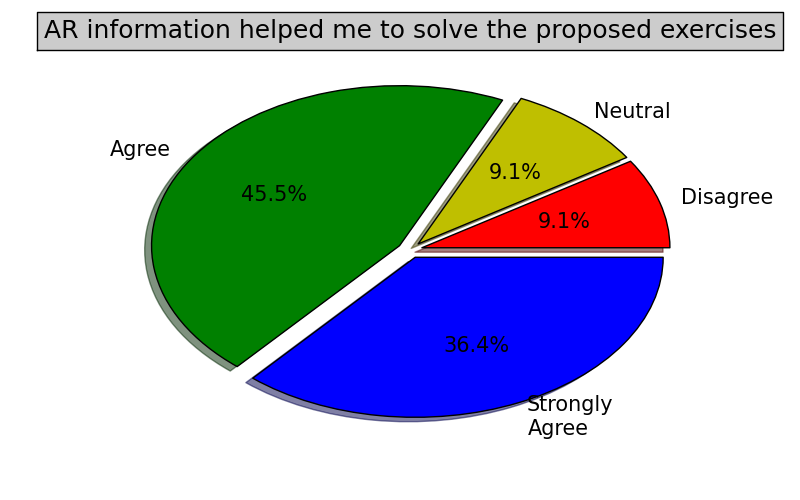
\includegraphics[width=0.47\textwidth]{img/survey/q6.png}\label{fig:survey:q6}}
  \subfigure{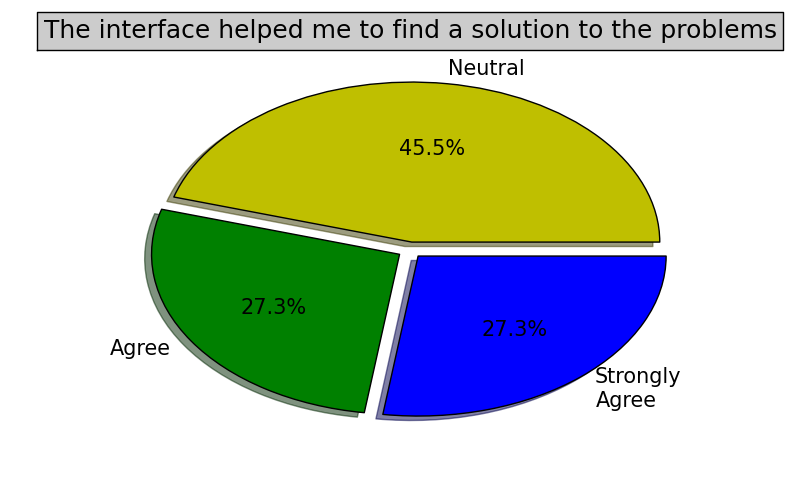
\includegraphics[width=0.47\textwidth]{img/survey/q7.png}\label{fig:survey:q7}}
  \caption{Survey questions, topic: interface exercises}
\end{figure}

One of the first observations is related to the progressive learning
process of the participants during the experiment. Most of them have
difficulties understanding the mechanics of the firsts two exercises
and serious mistakes are a very common event. However, they show an
important progress when solving the lasts problems, where nearly all
the mistakes are of minor importance. Further explanations were
required at the beginning of the session but as the participants
continued with it they progressively improve their problem solving
skills. For this reason, as seen in~\fig{fig:survey:q4}, the common
opinion is that the exercises are easy to solve.

The great majority of assistants agree that the combination of
Augmented Reality with the block\hyp{}world analogy provided a good
interface to solve the exercises. Their opinion is observed in the
questions in~\figs{fig:survey:q5}{fig:survey:q6}. Additionally,
more than half of the participants commented positively regarding to
how the interface helps to find out a solution to the exercises. This
question is found in~\fig{fig:survey:q7}. As a conclusion, the
application of these concepts was beneficial for the learning process.

\begin{figure}
  \centering
  \subfigure{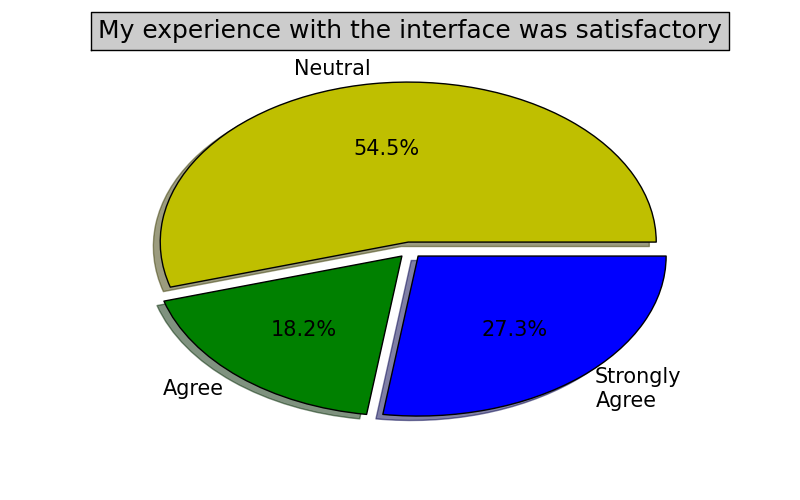
\includegraphics[width=0.47\textwidth]{img/survey/q9.png}\label{fig:survey:q9}}
  \subfigure{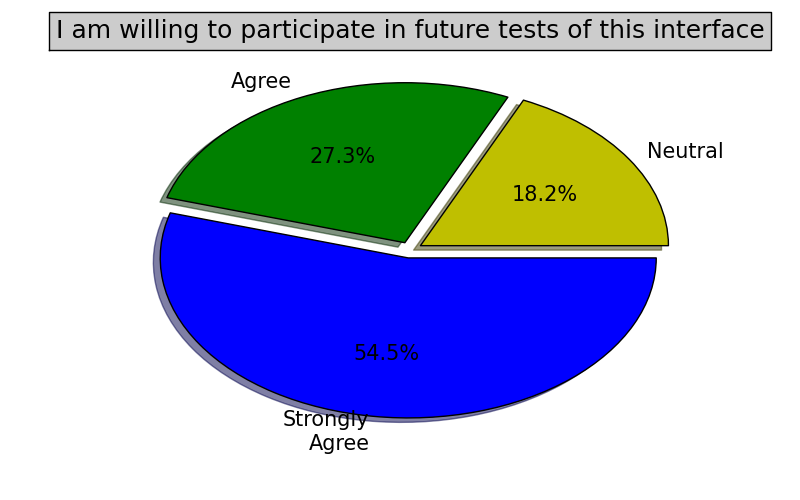
\includegraphics[width=0.47\textwidth]{img/survey/q11.png}\label{fig:survey:q11}}
  \subfigure{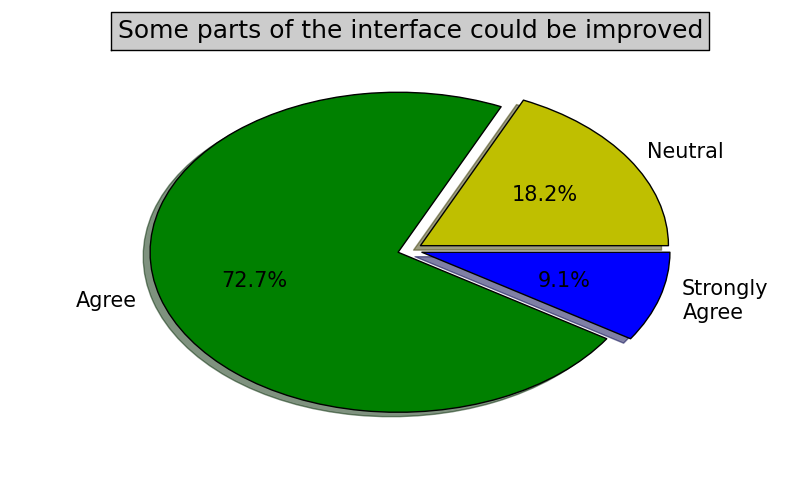
\includegraphics[width=0.47\textwidth]{img/survey/q10.png}\label{fig:survey:q10}}
  \caption{Survey questions, topic: general experience}
\end{figure}

Additionally, 45.5\% of the students have a good experience with the
interface and 81.8\% are willing to participate in future experiments,
this can be seen in more detail in~\fig{fig:survey:q9} and
in~\fig{fig:survey:q11}. Many of them complained about the fact that
every time a mistake is made the whole process should be restarted
from a valid initial state. This is one of the main critiques as
observed by the question in~\fig{fig:survey:q10} where 81.8\% of the
participants believe that several parts of the interface could be
improved. This interface's comportment underlies two intentions. The
first is to verify that the assistant can solve the each problem as a
whole and not just part of it; and the second is to use repetitions as
a form of punishing errors. Nevertheless, the opinions towards the
interface are positive.

\begin{figure}
  \centering
  \subfigure{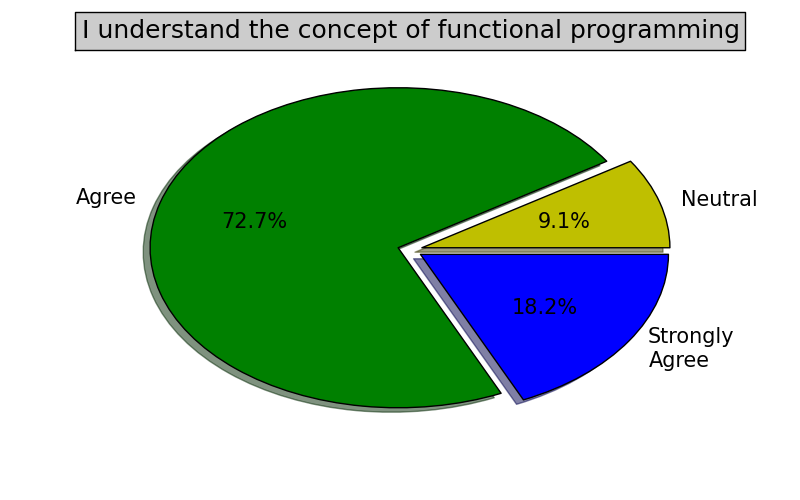
\includegraphics[width=0.47\textwidth]{img/survey/q1.png}\label{fig:survey:q1}}
  \subfigure{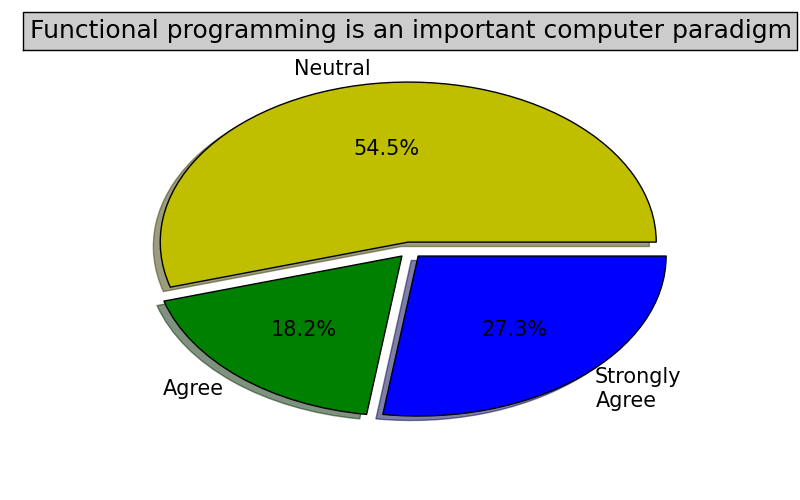
\includegraphics[width=0.47\textwidth]{img/survey/q3.png}\label{fig:survey:q3}}
  \subfigure{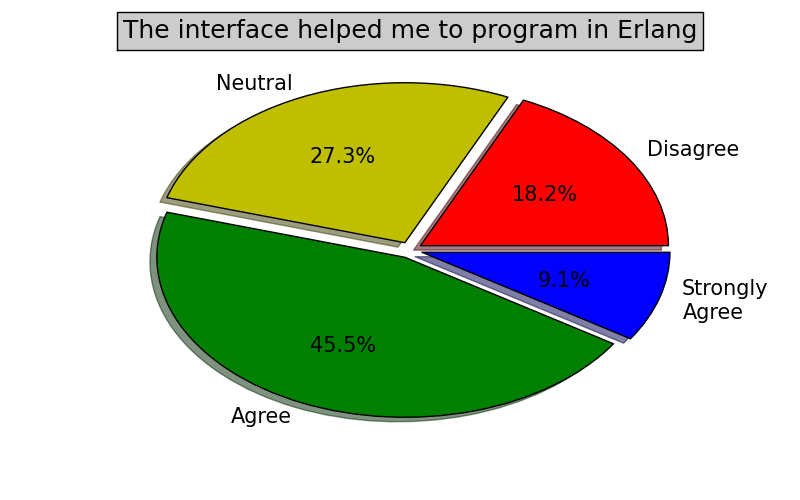
\includegraphics[width=0.47\textwidth]{img/survey/q8.png}\label{fig:survey:q8}}
  \subfigure{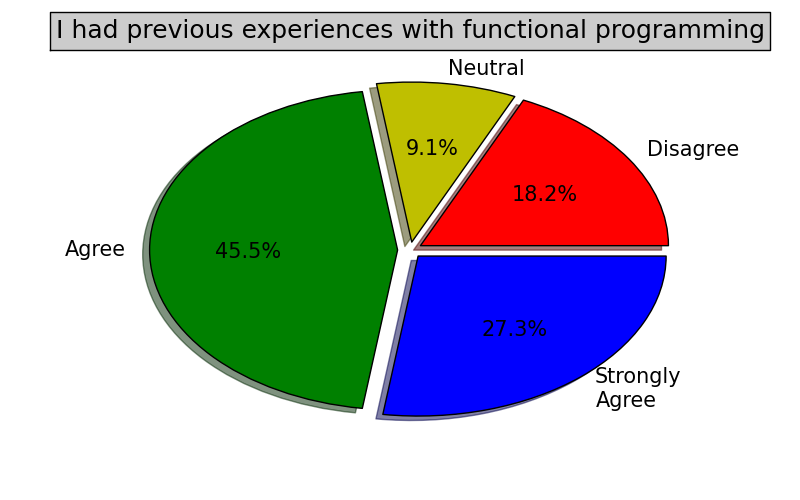
\includegraphics[width=0.47\textwidth]{img/survey/q2.png}\label{fig:survey:q2}}
  \caption{Survey questions, topic: functional programming}
\end{figure}

In the field of functional programming a curious event was observed.
Even though most of the participants have notions of understanding the
concept of functional programming, 54.5\% of them are neutral towards
considering it an important computer paradigm, this is shown
by~\fig{fig:survey:q1} and~\fig{fig:survey:q3}. This is a consequence
of colleges curriculum where \emph{object oriented} languages are
pervasive letting no space to different approaches. Therefore,
computer science students do not appreciate the benefits of using
functional programming languages.

Finally, only a small number of students, 18.2\%, commented that the
interface did not help them to learn \erlang, as shown
by~\fig{fig:survey:q8}. This remarkable development can occur by
several reasons. The first explanation relates the brevity of the
experiment where the proposed didactic phases are not followed.
However, longer sessions are expected to give a better understanding
of the \erlang-interface analogy and then transferring a
better training to the students. A second explanation is related to
participants' previous skills. As observed in~\fig{fig:survey:q2},
some students never have any contact with a functional programming
language, thus, making more difficult the process of learning. In
general, the feedback received in this point is very positive towards
the interface's purposes.

%%-*-latex-*-

\section{Conclusion}

\vestige is a tangible interface to help students in the process of
learning recursion which main interaction mechanism consists of
arranging blocks by forming stacks. The interface is accompanied by a
didactic methodology where the learning is acquired progressively.
Finally, users of the interface who follow the methodology are
expected to transfer their learning to write \erlang programs.

Many technical efforts have been spent in order have the application
run on \textsf{GNU/Linux} and be licensed as open source, so the
interested researchers may benefit from the freedom to study it, use
it, modify it and redistribute it under the same terms.

An initial experimental session involving several computer science
students was conducted. A progressive learning was observed in the
majority of the participants, their skills improved as they advanced
through the proposed exercises. They were also asked to complete
an exploratory survey in order to gather their opinions and feedback.
In general, positive answers were collected among all the
participants concluding a successful pilot study.

A subsequent observation of this process suggests that even though
a great number of students have notions of understanding the
concept of functional programming only a minority considers it an
important computer paradigm. Computer science programs curricula
should emphasize more on teaching its benefits and importance.

The positive answers gathered from the participants are an incentive
to take the interface further. The next logical step is to test
with a group of recursion students the whole system by following the
proposed didactic phases for progressive learning.

%*******************************************************************************
\subsection{Scope \& Limitations}
%*******************************************************************************

This study is limited by several methodological and practical
restrictions. The interface focuses on problems that stress the use of
lists and their structural order. For this reason, many algorithms are
left out the scope of the interface and can not be simulated.
Nevertheless, some of these limitations are planned to be solve in
possible future works.

The first of these limitations lies in the type of recursion used.
In short, only algorithms coded in \emph{tail recursion} form can be
simulated in the interface. Tail recursion implies that the last
operation of the function is a recursive call and for this reason,
this kind of algorithms require the use of extra features such as a
\emph{control stack}. A future solution is planned in order to
overcome this impediment.

Problems that require arithmetic operations are also out of the scope
of the interface. For this reason, simple exercises such as
\emph{fibonacci} or \emph{factorial} can not be implemented.

Finally, the solution must define only one complete function. A
function is complete when it is valid for every possible input data.
An example of an incomplete function is shown
in~\fig{fig:code:firstg}. In this case, the use of \erlang
\emph{atoms} is required for it to be valid on empty lists. In
addition, only single functions are supported because the system
represents only one function at the time.

%*******************************************************************************
\subsection{Future Work}
%*******************************************************************************

In the technical aspect, future work would involve increasing the
application's domain by exceeding its limitations. An initial idea
consists in the simulation of the \emph{control stack}. This stack
is where data of undergoing function calls are stored. This would
required adding special markers where the \push and \pop operations
are done top\hyp{}down as a contrast of normal stacks that are filled
bottom\hyp{}up).

Additionally, more exercises could be implemented. Initial ideas
suggests that problems such as \emph{Hanoi Towers} or different
versions of \emph{Insertion Sort} could be easily programmed. However,
this depends on extra features such as allowing multiple actions per
step, which are not currently implemented.

Finally, further experiments must be done in order to validate the
effectiveness of the didactic phases. This requires to conduct the
tests along with the students of a real class of functional
programming.


\newpage\addcontentsline{toc}{section}{References}
\bibliographystyle{plain}
\bibliography{recursion,tui}

\end{document}
